%  !TeX  root  =  user_guide.tex

%\section{OpenStreetMap Plugin}\label{plugins_osm}
\section{Extension OpenStreetMap}\label{plugins_osm}

% when the revision of a section has been finalized, 
% comment out the following line:
% \updatedisclaimer

%In recent years the OpenStreetMap project has gained popularity because in many countries no free geo data such as digital roadmaps are available. Target of the OSM project is to create a free editable map of the world from GPS data, aerial photography or simply from local knowledge. To support this idea QGIS provides a plugin that enables its users to work with OSM data.
Ces dernières années, le projet OpenStreetMap a gagné en popularité, car dans beaucoup de pays, aucune donnée géographique gratuite telle que le réseau routier n'est disponible. L'objectif du projet OSM est de créer une carte du monde éditable à partir de données GPS, de photographies aériennes ou tout simplement des connaissances locales du terrain. Pour soutenir ce projet, QGIS fournit une extension qui permet aux utilisateurs de travailler avec les données OSM.

%The plugin provides all basic functionalities for OSM data manipulation, such as data loading, importing, saving, downloading, editing and uploading data back to the OpenStreetMap server. While implementing OSM plugin an inspiration was taken from existing OSM data editors. The purpose was to combine their functionalities to get the best possible result.
L'extension fournit toutes les fonctionnalités de base pour manipuler les données OSM : chargement des données, import, sauvegarde, téléchargement en local, édition et téléchargement des données vers le serveur OpenStreetMap. Cette extension s'inspire des éditeurs OSM existants. Le but est de combiner leurs fonctionnalités pour obtenir le meilleur résultat possible.

%The following section gives a brief introduction to principles of the OSM project. If you are not interested in information on OSM just skip the next section. Parts of the following paragraphs are copied from the OpenStreetMap web site at \url{http://www.openstreetmap.org}.
La section suivante donne une brève introduction aux principes du projet OSM. Si vous n'êtes pas intéressé par des informations sur OSM, passez directement à la section suivante. Certaines parties des paragraphes suivants proviennent du site internet d'OpenStreetMap, \url{http://www.openstreetmap.org}.

%\minisec{The OpenStreetMap project}
\minisec{Le projet OpenStreetMap}

%OpenStreetMap is a project to create a free editable map of the world. The maps are created using data from portable GPS devices, aerial photography, other free sources or simply from local knowledge. The project was started because most maps have legal or technical restrictions on their use, holding back people from using them in creative, productive, or unexpected ways. Both rendered images and the vector dataset of OSM are available for download under a Creative Commons Attribution ShareAlike 2.0 licence.
Le projet OpenStreetMap a pour objectif de créer une carte libre et gratuite du monde. Les cartes sont créées à partir d'appareils GPS portables, de photographies aériennes et d'autres ressources libres ou simplement grâce aux connaissances locales. Le projet a été lancé sur le constat que l'utilisation de la plupart des cartes se heurte à des contraintes légales ou techniques, empêchant les gens de les utiliser de manière créative, productive ou autre. Les rendus image ou vectoriel des données OSM sont disponibles au téléchargement sous la licence Creative Commons Attribution ShareAlike 2.0.

\begin{figure}[ht]
   \centering
   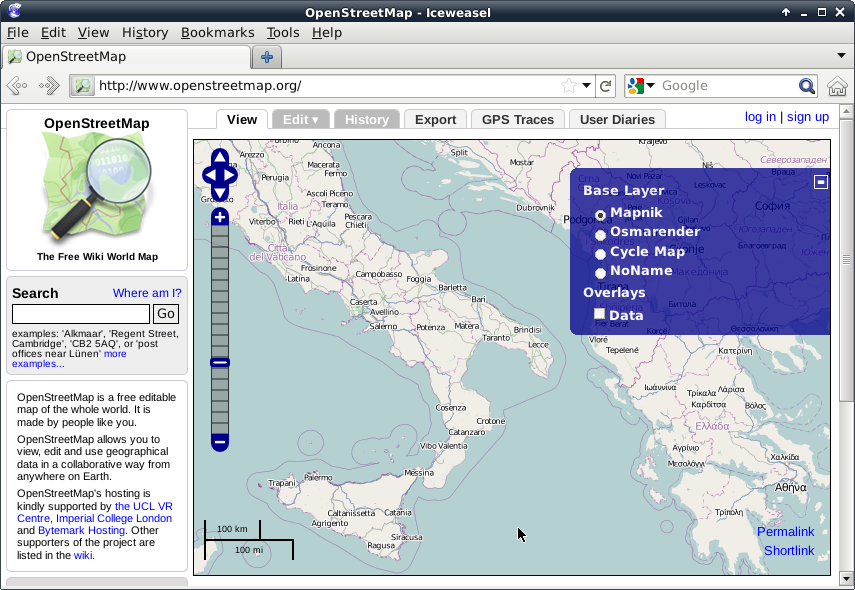
\includegraphics[clip=true, width=10cm]{osmweb}
   %\caption{OpenStreetMap data in the web \nixcaption}\label{fig:osmweb}
   \caption{Données OpenStreetMap sur Internet \nixcaption}\label{fig:osmweb}
\end{figure}

%OpenStreetMap was inspired by sites such as Wikipedia - the map display (see Figure \ref{fig:osmweb}) features a prominent \tab{Edit} tab and a full revision history is maintained. Registered users can upload GPS track logs and edit the vector data using the given editing tools.
OpenStreetMap s'est inspiré de sites tel que Wikipedia - l'affichage de la carte (voir Figure \ref{fig:osmweb}) s'accompagne d'un onglet \tab{Modifier} et un historique complet des changements est gardé. Les utilisateurs enregistrés peuvent envoyer leurs traces GPS et éditer les données vectorielles en utilisant les outils fournis.

%OSM data primitive is an object class that can be stored via the API in the server. The three supported types of data are: \textbf{Node}, \textbf{Way} and \textbf{Relation}. 
La primitive des données OSM est une classe objet qui peut être stockée sur le serveur via une API. Les trois types de données existants sont : le \textbf{noeud}, la \textbf{trace} (Way) et la \textbf{relation}.

\begin{itemize}[label=--]
%\item[A node} is a latitude/longitude pair of coordinates. It is used as building a block for other features and as a feature itself (Points Of Interest), if they are tagged as required. 
\item[Un noeud] est une paire de coordonnées latitude/longitude. Il sert de brique de base pour les autres entités, étant lui-même une entité (Point d'intérêt - POI) s'ils sont étiquetés correctement.
%\item[A way} is a list of at least two nodes that describe a linear feature such as a street, or similar. Nodes can be members of multiple ways.
\item[Une trace] est une liste d'au moins deux noeuds qui décrit une entité linéaire telle qu'une rue. Les noeuds peuvent appartenir à plusieurs traces.
%\item[A relation} is a group of zero or more primitives with associated roles. It is used to specify relationships between objects, and may also model an abstract object. 
\item[Une relation] est un groupe composé de zéro primitive ou plusieurs associées à des rôles. C'est utilisé pour définir des relations entre les objets, mais peut également modéliser un objet abstrait.
\end{itemize}

%Several different logical features in a common map ('Point Of Interest', 'Street', 'Tram Line', 'Bus Stop' etc.) are defined by these primitives. Map features are well-known in the OSM community and are stored as tags, based of a key and a value. OSM is usually distibuted in XML format. XML payload is used for the communication with the OSM server as well.
Plusieurs différentes entités logiques sur une carte classique (Point d'intérêt, rue, ligne de tramway, arrêt de bus, etc.) sont définies par ces primitives. Les entités cartographiques sont bien connues dans la communauté OSM et sont stockées en tant que \og tag\fg (étiquette), basé sur une clé et une valeur. Les données OSM sont en général distribuées au format XML. Un \og XML payload\fg est également utilisé pour la communication avec le serveur OSM.

%\minisec{QGIS - OSM Connection}\label{qgis-osm-connection}
\minisec{Connexion QGIS - OSM}\label{qgis-osm-connection}

%The first part of this section describes how OSM data primitives are displayed in QGIS vector layers. As written above, OSM data consist of Nodes, Ways and Relations. In QGIS they are displayed in three diffrent layer types: Point layer, Line layer and Polygon layer. It's not possible to remove any of these layers and work with the other ones.
La première partie de ce paragraphe décrit de quelle manière les primitives des données OSM sont affichées dans des couches vectorielles QGIS. Comme il est précisé ci-dessus, les données OSM se composent de noeuds, de traces et de relations. Dans QGIS, elles sont affichées dans trois couches de type différent : couche de points, de lignes et de polygones. Il est impossible de retirer l'une de ces couches et de travailler avec les autres.


\begin{itemize}[label=--]
%\item A \textbf{Point layer} displays all features of type Node that stands alone. That means that only Nodes that are not included in any Way belongs to the Point layer.
\item[Une couche de points ] affiche toutes les entités de type noeud isolé. Ce qui signifie que seuls les noeuds qui ne sont pas inclus dans une trace appartiennent à la couche de points.
%\item A \textbf{Line layer} displays those OSM features of type Way that are not closed. That means, none of these Ways starts and ends with the same Node.
\item [Une couche de lignes] affiche les entités OSM de type trace qui ne sont pas fermées. Cela signifie qu'aucune de ces traces ne commence et finit par le même noeud.
%\item A \textbf{Polygon layer} displays all Ways that are not included in Line layer.
\item[Une couche de polygones] affiche toutes les traces qui ne sont pas incluses dans la couche de lignes.
\end{itemize}

%OpenStreetMap has one more data primitive except for the three mentionedabove. This is called \textbf{Relation}. There is purposely no vector layer to display Relations. A Relation defines relation between any number of data primitives. After Point, Line or Polygon is identified on a map, the plugin shows a list of all relations, the identified feature is part of.
En plus des trois cités ci-dessus, OpenStreetMap possède un dernier type de données, il s'agit des \textbf{Relations}. Il n'y a pas de couche vectorielle dédiée à la représentation des relations. Une relation définit la relation entre n'importe quel nombre de primitives. Dès qu'un point, une ligne ou un polygone est identifié sur la carte, l'extension affiche la liste de toutes les relations auxquelles l'entité appartient.

%Challenging was to design the connection between OSM data and the standard QGIS editing tools. These tools are made to edit a single vector layer at a time, no matter of what feature types it displays. This means that if OSM data are loaded to QGIS through the plugin, you could (theoretically) edit Point layer, Line layer or Polygon layer with these standard tools separately.
Ce fut une vraie épreuve de définir la connexion entre les données OSM et les outils standards d'édition de QGIS. Ces outils sont faits pour éditer chaque couche vectorielle séparément, quel que soit le type d'entités. Ce qui signifie que si des données OSM sont chargées dans QGIS via l'extension, vous pourriez théoriquement éditer les couches de points, de lignes et de polygones avec ces outils standards séparément.

%The problem is, that Line layer consists of two different types of OSM features - Ways and Nodes. Why? Because in OSM format a Way is composed of Nodes. If you start editing a Line layer and change the shape of some line, your action must affect not only the OSM Way but also the OSM Nodes that are part of it.
Le problème est que la couche de ligne est composée de deux types différents d'entités OSM - des traces et des noeuds. Pourquoi ? Parce que dans le format OSM, une trace est composée de noeuds. Si vous commencez à éditer une couche de ligne et que vous changez la forme d'une ligne, votre action doit affecter non seulement la trace OSM, mais également les noeuds qui la composent.

%QGIS standard editing tools cannot tell the OSM provider, which members of which line has changed and how. It can tell only what's the new geometry of which line, and that's not enough to propagate changes to the OSM database correctly. The Line layer does also not know the identifiers of the line members. The same problem occurs when you try to edit the Polygon layer.
Les outils d'édition standards de QGIS ne peuvent pas dire au fournisseur OSM quels sont les noeuds qui ont changé et comment. Ils peuvent seulement dire quelle est la nouvelle géométrie de chaque ligne, mais ce n'est pas suffisant pour propager les changements à la base de données OSM correctement. La couche ligne ne connait pas non plus les identifiants des points des noeuds qui la constituent. Le même problème apparaît lorsque vous essayez d'éditer la couche de polygones.

%For this reason, the OSM plugin need its own tools for editing OSM data. While they are used, the OSM layers can be changed correctly. The Plugin editing tools consists of tools for Point, Line, Polygon and Relation creation, deletion and moving.
Pour ces raisons, l'extension OSM a besoin de ses propres outils d'édition des données OSM. Tant qu'ils sont utilisés, les couches OSM peuvent être éditées correctement. Les outils d'édition de l'extension comprennent des outils pour la création, la suppression et le déplacement de points, de lignes, de polygones et de relations.

%\textbf{Note:} To create a connection between the OSM plugin and standard editing tools, changes in QuantumGIS core code would be necessary.
\textbf{Note :} Pour créer une connexion entre l'extension OSM et les outils standards d'édition, des modifications dans le code principal de QGIS seraient nécessaires. 

%The OpenStreetMap plugin is a core plugin inside QGIS. If you have python support enabled, the 'OpenStreetMap' plugin can be selected in the Plugin Manager as described in section \ref{sec:load_core_plugin}). 
L'extension OpenStreetMap fait partie des extensions principales de QGIS. Si le support pour Python est activé, l'extension \og OpenStreetMap\fg peut être sélectionnée dans le Gestionnaire d'extensions tel que décrit dans la section \ref{sec:load_core_plugin}).

%\subsection{Basic user interface}
\subsection{Interface utilisateur de base}

%The first time the OSM plugin is started (and after the first data are loaded), several new OSM plugin icons appear in the QGIS toolbar menu together with new graphical components as shown in Figure \ref{fig:osmwidget}:
Au premier lancement de l'extension OSM (et une fois les premières données chargées), plusieurs nouvelles icônes OSM avec de nouveaux composants graphiques apparaissent dans la barre d'outils d'OSM, comme on peut le voir sur la figure \ref{fig:osmwidget} :

\begin{figure}[ht]
   \centering
   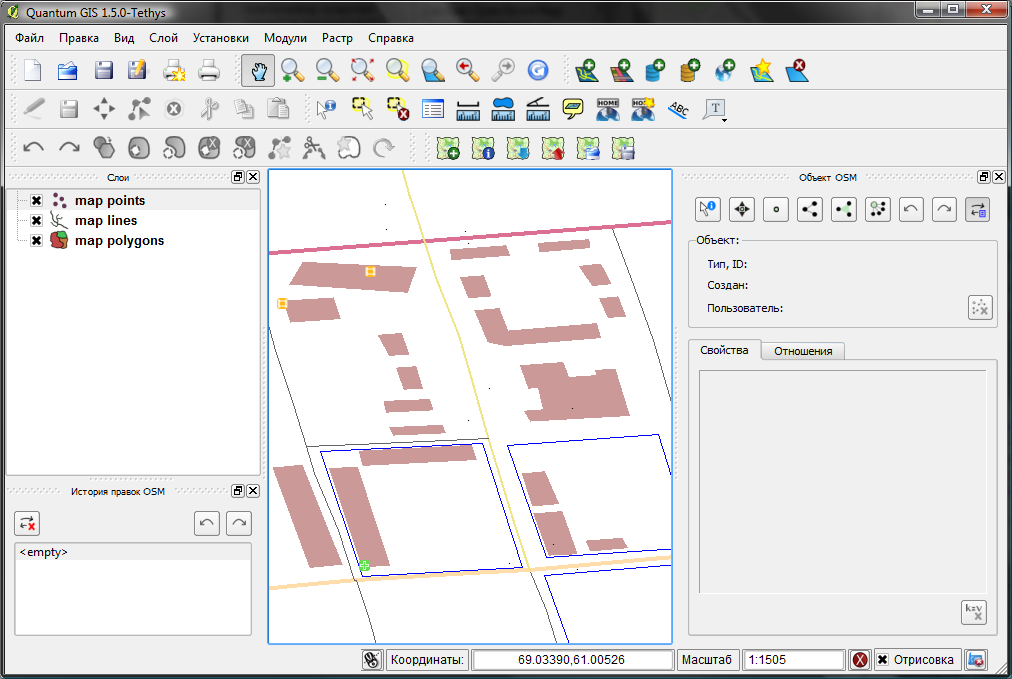
\includegraphics[clip=true, width=10cm]{osm_widgets}
   %\caption{OSM plugin user interface \nixcaption}\label{fig:osmwidget}
   \caption{Interface utilisateur de l'extension OSM \nixcaption}\label{fig:osmwidget}
\end{figure}

%\minisec{OSM Features widget}
\minisec{Widget Entité OSM}

%The OSM Feature widget helps to identify OSM features. It shows basic information on feature type and identifier as well as info on who has when changed a feature. The OSM Feature widget also provides all editing tools (in the top part of it). More information on those tools can be found in the sections below. The widget is initially disabled. It activates itself after successfull loading some OSM data.
L'outil d'entité OSM aide à identifier les entités OSM. Il montre les informations de base sur le type et l'identifiant de l'entité sélectionnée ainsi que l'historique des changements avec leur auteur. L'outil donne également accès à tous les outils d'édition (dans sa partie supérieure). Vous trouverez plus d'informations sur ces outils dans la section suivante. L'outil est initialement désactivé, il apparait automatiquement dès que des données OSM sont chargées avec succès.

%\minisec{OSM Undo/Redo widget}
\minisec{Widget Editer l'historique OSM}

%This Undo/Redo widget is used to undo and redo edit actions. It consists not only of a classical Undo and Redo button, it also shows a list with a brief description of the edit actions that were done. The OSM Undo/Redo widget is initially closed. You can show it using a button on OSM Feature widget.
Cet outil Éditer l'historique d'OSM est utilisé pour annuler ou refaire des actions d'édition. Il s'agit non seulement d'un classique bouton Annuler/Refaire mais il liste également les actions d'éditions effectuées avec une courte description. Ce widget est initialement fermé, vous pouvez le faire apparaître en cliquant sur un bouton de l'outil Entité d'OSM.

%\minisec{Toolbar menu icons}
\minisec{Icônes de la barre de menu}

\begin{description}
%\item \toolbtntwo{osm_load}{Load OSM from file :] is used to load data from a special OpenStreetMap XML file.
\item \toolbtntwo{osm_load}{Charger OSM depuis un fichier} est utilisé pour charger des données à partir d'un fichier XML spécial OpenStreetMap (.osm)
%\item \toolbtntwo{osm_featureManager}{Show/Hide OSM Feature Manager} is used to show or hide the OSM Feature widget. The OSM Feature widget is a panel that helps with OSM feature identification and with OSM data editing.
\item \toolbtntwo{osm_featureManager}{Afficher/Cacher le gestionnaire d'entités OSM} est utilisé pour montrer ou cacher le widget Entité OSM. Il s'agit d'un panneau qui aide à l'identification des entités OSM et l'édition des données OSM.
%\item \toolbtntwo{osm_download}{Download OSM data} is used to download data from the OpenStreetMap server.
\item \toolbtntwo{osm_download}{Télécharger des données OSM} est utilisé pour télécharger des données depuis le serveur OpenStreetMap.
%\item \toolbtntwo{osm_upload}{Upload OSM data} is used to upload changes (on current data). 
\item \toolbtntwo{osm_upload}{Charger des données OSM} est utilisé pour charger les changements (effectués sur les données téléchargées). 
%\item \toolbtntwo{osm_import}{Import data from a layer} is used to import data from a vector layer. At least one vector layer must be loaded and current OSM data must be selected.
\item \toolbtntwo{osm_import}{Importer des données depuis une couche} est utilisé pour importer des données depuis une couche vecteur. Au moins une couche vectorielle doit être chargée et les données OSM courantes doivent être sélectionnées.
%\item \toolbtntwo{osm_save}{Save OSM to file} is used to save OSM data back to an XML file.
\item \toolbtntwo{osm_save}{Sauvegarder OSM sur un fichier} est utilisé pour enregistrer des données OSM à nouveau dans un fichier XML.
\end{description}

%More detailed information on all the widgets, buttons and dialogs can be found in appropriate sections of this plugin section according to their functionality (editing, identification, etc.).
Des informations plus détaillées sur tous les outils, boutons et fenêtres se trouvent dans les sections correspondant à leur fonction (édition, identification, etc.).

%\subsection{Loading OSM data}
\subsection{Charger des données OSM}

%The first action that should be done after starting the OSM Plugin is opening data from an OSM file. OSM data can be import as shapefile or downloaded directly from the OpenStreetMap server. Here we are focusing on the first mentioned method.
La première action qui devrait faire suite au lancement de l'extension OSM est l'ouverture de données depuis un fichier OSM. Les données OSM peuvent être importées comme shapefile ou directement téléchargées depuis le serveur OpenStreetMap. Nous allons nous focaliser ici sur la première méthode mentionnée.

%To load data from a file use the \toolbtntwo{osm_load}{Load OSM from file} icon. If there is no such button, maybe someone disabled OpenStreetMap toolbar in your QGIS instalation. You can enable it again selecting \mainmenuopt{Settings} > \mainmenuopt{Toolbars} > \dropmenuopt{OpenStreetMap}.
Pour charge des données depuis un fichier, cliquez sur l'icône \toolbtntwo{osm_load}{Charger OSM depuis un fichier}. S'il n'y a pas de tel bouton, la barre d'outils OpenStreetMap n'est peut-être pas activée dans QGIS. Vous pouvez faire apparaître en sélectionnant \mainmenuopt{Vue} > \mainmenuopt{Barres d'outils} > \dropmenuopt{OpenStreetMap}.

\begin{figure}[ht]
   \centering
   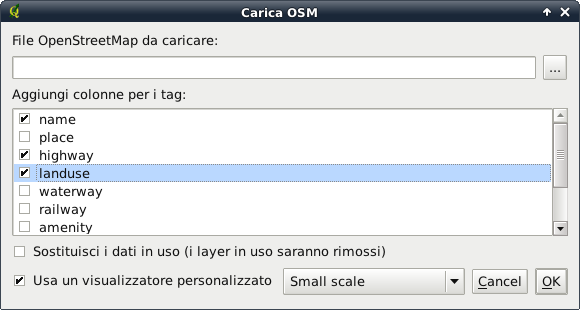
\includegraphics[clip=true, width=10cm]{osmloaddialog}
   %\caption{Load OSM data dialog \nixcaption}\label{fig:osmload}
   \caption{Fenêtre de chargement de données OSM \nixcaption}\label{fig:osmload}
\end{figure}

%Purpose of its elements is explained below.
Le but de chacun de ses éléments est expliqué ci-dessous :

\begin{description}
%\item[OpenStreetMap file to load :] Click on the button to select the .osm file you want to load data from.
\item[Fichier OpenStreetMap à charger :] Cliquez sur le bouton pour sélectionner le fichier .osm dont vous voulez charger les données.
%\item[Add columns for tags :] This option determines a connection between OSM and QGIS data. Each feature of OSM data has some tags (pairs of key and value), that define the feature properties. Each feature of a QGIS vector layer also has its attributes (key and value). With this option you can define which properties of OSM objects should be visible when displaying detailed information about QGIS features.
\item[Ajouter des colonnes pour les tags :] Cette option définit une connexion entre des données OSM et QGIS. Chaque entité de données OSM possède une série de tags (une paire clé valeur) qui définit les propriétés de l'entité. Chaque entité d'une couche vectorielle QGIS possède également ses attributs (clé et valeur). Avec cette option, vous pouvez définir quelles propriétés des objets OSM seront visibles lorsque vous affichez les informations détaillées sur les entités QGIS.
%\item[Replace current data :] Checking this option means that new data should replace current data the user is working with. Layers of current data will be removed and new ones will be loaded. When loading OSM data for the first time, this option is not active, because there is nothing to replace.
\item[Remplacer les données actuelles :] Cocher cette option signifie que les nouvelles données doivent remplacer celles utilisées actuellement. Les couches des données actuelles seront supprimées et les nouvelles chargées. Lorsque vous chargez des données OSM pour la première fois, cette option n'est pas active, car il n'y a rien à remplacer.
%\item[Use custom renderer :] This option determines how many details of the map will be used. There are three pre-defined OSM styles for map displaying. Use \button{Small scale} if you want to view OSM data at low level, to see all details and to edit something. If not you can use \button{Medium scale} or \button{Large scale}. QGIS \CURRENT doesn't support changing the renderer style dynamically.
\item[Utiliser un rendu prédéfini :] Cette option détermine combien de détails de la carte seront utilisés. Il y a trois styles OSM prédéfinis pour la carte. Utilisez \button{Petite échelle} si vous souhaitez afficher des données OSM à un petit niveau, voir tous les détails et éditer les données. Sinon vous pouvez utiliser \button{Échelle intermédiaire} ou \button{Grande Échelle}. QGIS \CURRENT ne permet pas de changer dynamiquement ces styles de rendu.
\end{description}

%Click \button{Ok} to load your data. If this is the first time OSM file is loaded, the plugin must first parse the database. This may take few seconds or minutes - it depends on the amount of loaded data.
Cliquez sur \button{Ok} pour charger vos données. S'il s'agit du premier chargement de données OSM, l'extension doit d'abord parcourir la base de données. Cela peut prendre quelques secondes ou minutes selon la quantité de données à charger.

%\subsection{Viewing OSM data}
\subsection{Visualiser des données OSM}

%After OSM data are loaded, you can identify map features using the appropriate tool. Use the \toolbtntwo{osm_identify}{Identify feature} button on the top-left of OSM Feature widget. Using this tool you can easily explore all map objects. When the mouse cursor is placed over an object, you can see all information on it directly in the OSM Feature widget. There is also a dynamic rubberband displayed on the map so that the user is able to determine which feature is currently identified.
Une fois les données OSM chargées, vous pouvez identifier les entités cartographiques en utilisant l'outil approprié. Utilisez le bouton \toolbtntwo{osm_identify}{Identifier l'entité} en haut à gauche de l'outil Entité OSM. Avec cet outil vous pouvez facilement explorer tous les objets cartographiques. Quand le curseur de la souris est placé sur un objet, vous pouvez voir toutes les informations le concernant directement dans l'outil Entité OSM. Il y a également une étiquette qui s'affiche sur la carte pour que l'utilisateur puisse déterminer l'entité en cours d'identification.

%The \tab{Properties} tab of the widget contains of all feature tags. Clicking on the \tab{Relation} tab shows you a list of all relations connected with identified feature.
L'onglet \tab{Propriétés} de l'outil contient tous les tags de l'entité. En cliquant sur l'onglet \tab{Relation}, une liste de toutes les relations auxquelles l'entité appartient apparaît.

%If you want to hold a feature for a while to be able to read its properties and relations, move the mouse cursor at the same time, try left-clicking while you are over the feature. Identification process will stop until next left-clicking.
Si vous souhaitez prendre le temps de lire les propriétés et les relations d'une entité et déplacer simultanément le curseur de la souris, faites un clic gauche sur l'entité. Le processus d'identification au passage de la souris s'arrêtera jusqu'au prochain clic-gauche.

%Sometimes there are more than one feature at a point where left-clicking was performed. This happens especially when clicking on cross-roads or if you didn't zoom enough into the map. In this situation only one of such features is identified (and marked with the rubberband) but the plugin remembers all of them. Then (still in the pause mode) you can change identified features cyclical with right-clicking.
Il y a parfois plus d'une entité à l'endroit du point cliqué. Cela arrive surtout lorsque l'on clique sur un croisement de routes ou lorsque vous n'avez pas assez zoomé sur la carte. Dans ce cas, seule une entité est identifiée (et marquée par l'étiquette), mais l'extension les garde toutes en mémoire. Ensuite vous pouvez changer les entités identifiées de manière cyclique en faisant un clic droit.

%\subsection{Editing basic OSM data}
\subsection{Éditer des données OSM de base}

%In the title of this section 'basic data' means non-relation OSM features - nodes and ways. If you prefer reading information on relation editing, just skip this section and read the next one.
Dans le titre de cette section, \og données de base\fg signifie entités de type noeud ou trace, pas relation. Si vous souhaitez avoir des informations sur l'édition de relations, sautez cette section et passez à la suivante.
 
%Basic data editing is a key part of OSM Plugin. You can change property, position or shape of any existing basic feature. You can remove features or add new ones. All such changes on nodes and ways are remembered for comfortable usage of Undo/Redo operations and for easy upload of all changes to OpenStreetMap server.
L'édition des données de base est une partie clé de l'extension OSM. Vous pouvez changer la propriété, la position ou la forme de n'importe quelle entité de base existante. Vous pouvez en supprimer ou en ajouter de nouvelles. Toutes ces modifications sur les noeuds et les traces sont gardées en mémoire pour faciliter les opérations annuler/refaire et pour faciliter leur chargement sur le serveur d'OpenStreeMap.

%\minisec{Changing feature tags}
\minisec{Changer les tags d'une entité}

%Changing the property/tag of an OSM feature can be done directly in the table of feature tags. The Tags table of basic features can be found on the OSM Feature widget. Don't forget to identify feature first.
Changer une propriété/un tag d'une entité OSM peut être réalisé directement dans la table des tags de l'entité. Cette table des tags des entités de base se trouve dans l'outil Entité OSM. N'oubliez pas d'identifier une entité au préalable.

\begin{figure}[ht]
   \centering
   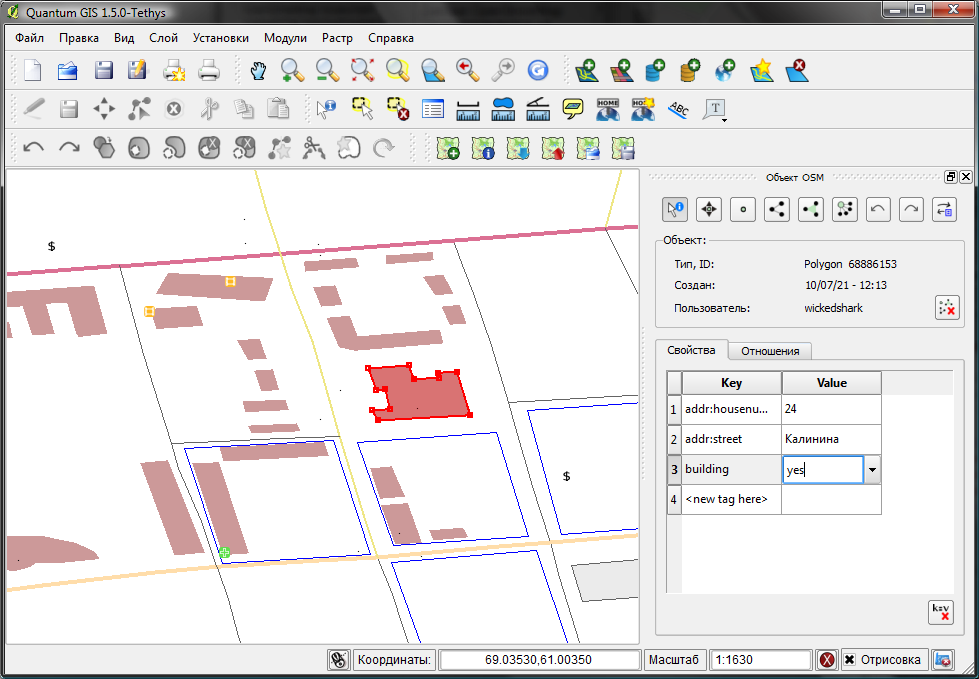
\includegraphics[clip=true, width=12cm]{osm_changefeaturetag}
   %\caption{Changing an OSM feature tag \nixcaption}\label{fig:osmchfeattag}
   \caption{Changer le tag d'une entité OSM \nixcaption}\label{fig:osmchfeattag}
\end{figure}

%If you want to change a tag value, just double-click in the appropriate row of column 'Value' and type or select a new value. If you want to remove a tag, click in its row, then use button \button{Remove selected tags} on the right bottom under the table.
Si vous souhaitez changer la valeur d'un tag, double-cliquez simplement sur la ligne appropriée de la colonne \og Valeur\fg et tapez ou sélectionnez une nouvelle valeur. Si vous souhaitez supprimer un tag, cliquez sur sa ligne puis utilisez le bouton \button{Supprimer les tags sélectionnés} situé en bas à droite sous la table.

%To add new tags just type its key and value into the last row of the table - where '<next tag value>' is written. Notice that you cannot change the key of an existing tag pair. For comfortable usage, there are some combo boxes of all existing tag keys and their typical values.
Pour ajouter de nouveaux tags, tapez simplement leur clé et leur valeur dans la dernière ligne de la table - où '<next tag value>' est écrit. Notez que vous ne pouvez pas changer la clé d'un tag existant. Pour une utilisation facilitée, il y a des listes déroulantes de toutes les clés de tag existantes et leur valeur typique.

%\minisec{Point creation}
\minisec{Création de point}

%For point creation there is a \toolbtntwo{osm_createPoint}{Create point} button on the OSM Feature widget. To create some points just click on the button and start clicking on the map. If your cursor is over some map feature, the feature is marked/identified immediately. If you click on the map when a line or polygon is marked, a new point is created directly on such line or polygon - as its new member. If your cursor is over an existing  point, new point cannot be created. In such case the OSM plugin will show following message:
Pour la création de points, il y a un bouton \toolbtntwo{osm_createPoint}{Créer un point} dans l'outil Entité OSM. Pour créer des points, cliquez simplement sur le bouton puis cliquez sur la carte. Si votre curseur se situe sur une entité déjà existante, elle se retrouve marquée/identifiée immédiatement. Si vous cliquez sur la carte quand une ligne ou un polygone est marqué, un nouveau point est créé directement sur la ligne ou le polygone, en tant que nouveau membre. Si votre curseur se trouve sur un point existant, aucun nouveau point ne peut être créé et l'extension OSM affichera le message suivant :

\begin{figure}[ht]
   \centering
   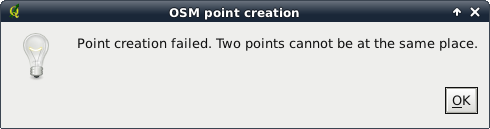
\includegraphics[clip=true, width=8cm]{osm_pointcreation}
   %\caption{OSM point creation message \nixcaption}\label{fig:osmpoicreat}
   \caption{Message de création de point OSM \nixcaption}\label{fig:osmpoicreat}
\end{figure}

%The mechanism of helping a user to hit the line or polygon is called snapping and is enabled by default. If you want to create a point very close to some line (but not on it) you must disable snapping by holding the \keystroke{Ctrl} key first.
Le mécanisme qui permet d'aider l'utilisateur à cliquer exactement sur une ligne ou un polygone s'appelle l'accrochage et est activé par défaut. Si vous voulez créer un point très près d'une ligne (mais pas dessus) vous devez d'abord désactiver l'accrochage en maintenant la touche \keystroke{Ctrl} enfoncée.

%\minisec{Line creation}
\minisec{Création d'une ligne}

%For line creation there is a \toolbtntwo{osm_createLine}{Create line} button on the OSM Feature widget. To create a line just click the button and start left-clicking on the map. Each of your left-clicks is remembered as a member vertex of the new line. Line creation ends when first right-click is performed. The new line will immediately appear on the map.
Pour la création de lignes, il y a un bouton \toolbtntwo{osm_createLine}{Créer une ligne} dans l'outil Entité OSM. Pour créer une ligne, cliquez simplement sur le bouton puis faites des clics gauches sur la carte. Chaque clic gauche est gardé en mémoire en tant que vertex de la nouvelle ligne. La création de la ligne se termine au premier clic droit. La nouvelle ligne apparaît alors immédiatement sur la carte.

%\textbf{Note :] A Line with less than two members cannot be created. In such case the operation is ignored.
\textbf{Note} : Une ligne composée de moins de deux membres ne peux pas être créée. Dans de tels cas, l'opération est ignorée.

%Snapping is performed to all map vertices - points from Point vector layer and all Line and Polygon members. Snapping can be disabled by holding the \keystroke{Ctrl} key.
L'accrochage se fait sur tous les vertex — les points des couches de points vectoriels et les membres de toutes les lignes et polygones. L'accrochage peut être désactivé en maintenant la touche \keystroke{Ctrl} enfoncée.

%\minisec{Polygon creation}
\minisec{Création d'un polygone}

%For polygon creation there is a \toolbtntwo{osm_createPolygon}{Create polygon} button on the OSM Feature widget. To create a polygon just click the button and start left-clicking on the map. Each of your left-clicks is remembered as a member vertex of the new polygon. The Polygon creation ends when first right-click is performed. The new polygon will immediately appear on the map. Polygon with less than three members cannot be created. In such case operation is ignored. Snapping is performed to all map vertexes - points (from Point vector layer) and all Line and Polygon members. Snapping can be disabled by holding the \keystroke{Ctrl} key.
Pour la création de polygones, il y a un bouton \toolbtntwo{osm_createPolygon}{Créer un polygone} dans l'outil Entité OSM. Pour créer un polygone, cliquez simplement sur le bouton puis faites des clic-gauche sur la carte. Chaque clic gauche est gardé en mémoire en tant que vertex du nouveau polygone. La création du polygone se termine au premier clic droit. Le nouveau polygone apparaît alors immédiatement sur la carte. Des polygones composés de moins de trois membres ne peuvent pas être créés. Dans de tels cas, l'opération est ignorée. L'accrochage se fait sur tous les vertex — les points des couches de points vecteurs et les membres de toutes les lignes et polygones. L'accrochage peut être désactivé en maintenant la touche \keystroke{Ctrl} enfoncée.

%\minisec{Map feature moving}
\minisec{Déplacement d'une entité cartographique}

%If you want to move a feature (no matter what type) please use the \toolbtntwo{osm_move}{Move feature} button from the OSM Feature widget menu. Then you can browse the map (features are identified dynamically when you go over them) and click on the feature you want to move. If a wrong feature is selected after your click, don't move it from the place. Repeat right-clicking until the correct feature is identified. When selection is done and you move the cursor, you are no more able to change your decision what to move. To confirm the move, click on the left mouse button. To cancel a move, click another mouse button.
Si vous souhaitez déplacer une entité (quel que soit son type), utilisez le bouton \toolbtntwo{osm_move}{Déplacer une entité} du menu de l'outil Entité OSM. Vous pouvez ensuite parcourir la carte (les entités sont alors identifiées dynamiquement au passage de la souris) et cliquez sur l'entité que vous souhaitez déplacer. Si la mauvaise entité est sélectionnée par ce clic, ne déplacez pas votre curseur. Refaites des clics droits jusqu'à ce que la bonne entité soit sélectionnée. Dès que la sélection est faite et que vous déplacez le curseur, vous ne pouvez plus changer d'entité à déplacer. Pour confirmer le déplacement, cliquez sur le bouton gauche de la souris. Pour l'annuler, cliquez sur un autre bouton de la souris.

%If you are moving a feature that is connected to another features, these connections won't be damaged. Other features will just adapt themselves to a new position of a moved feature. 
Si vous déplacez une entité qui est connectée à une autre, ces connexions ne seront pas endommagées. DLes autres entités s'adapteront d'elles-mêmes à la nouvelle position de l'entité déplacée.

%Snapping is also supported in this operation, this means: 
L'accrochage fonctionne également pour cette opération :

\begin{itemize}[label=--]
%\item When moving a standalone (not part of any line/polygon) point, snapping to all map segments and vertices is performed.
\item Lorsque vous déplacez un point seul (ne faisant pas partie d'une ligne ou d'un polygone), l'accrochage est réalisé sur tous les segments et vertex de la carte.
%\item When moving a point that is a member of some lines/polygons, snapping to all map segments and vertices is performed, except for vertices of point parents.
\item Lorsque vous déplacez un point membre de lignes ou de polygones, l'accrochage a alors lieu sur tous les segments et vertex de la carte, sauf ceux appartement aux lignes et polygones parents.
%\item When moving a line/polygon, snapping to all map vertices is performed. Note that the OSM Plugin tries to snap only to the 3 closest-to-cursor vertices of a moved line/polygon, otherwise the operation would by very slow. Snapping can be disabled by holding \keystroke{Ctrl} key during the operation.
\item Lorsque vous déplacez une ligne ou un polygone, l'accrochage sur tous les vertex de la carte est réalisé. Notez que l'extension OSM tente l'accrochage uniquement sur les 3 vertex les plus proches du curseur, l'opération serait très lente sinon. L'accrochage peut être désactivé en maintenant la touche \keystroke{Ctrl} enfoncée.
\end{itemize}

%\minisec{Map feature removing}
\minisec{Suppression d'une entité cartographique}

%If you want to remove a feature, you must identify it first. To remove an identified feature, use the \toolbtntwo{osm_removeFeat}{Remove this feature} button on the OSM Feature widget. When removing a line/polygon, the line/polygon itself is deleted, so are all its member points that doesn't belong to any other line/polygon.
Si vous souhaitez supprimer une entité, vous devez l'identifier au préalable. Ensuite pour la supprimer, utilisez le bouton \toolbtntwo{osm_removeFeat}{Supprimer l'entité} de l'outil Entité OSM. Lorsque vous supprimez une ligne ou un polygone, la ligne ou le polygone lui-même est supprimé, ainsi que tous les points qui le composent et qui ne font pas partie d'autres lignes ou polygones.

%When removing a point that is member of some lines/polygons, the point is deleted and the geometries of parent lines/polygons are changed. The new parent geometry has less vertices than the old one.
Lorsque vous supprimez un point qui est une partie de ligne ou de polygones, le point est supprimé et la géométrie des lignes ou polygones parents en est changée. La nouvelle géométrie a moins de vertex que l'ancienne.

%If the parent feature was a polygon with three vertexes, its new geometry has only two vertexes. And because there cannot exist polygon with only two vertices, as described above, the feature type is automatically changed to Line.
Si l'entité parente était un polygone composé de trois vertex, sa nouvelle géométrie en comprend seulement deux. Mais comme il ne peut exister de polygones à deux vertex, comme décrit précédemment, l'entité est automatiquement transformée en ligne.

%If the parent feature was a line with two vertexes, its new geometry has only one vertex. And because there cannot exist a line with only one vertex, the feature type is automatically changed to Point.
Si l'entité parente était une ligne avec deux vertex, sa nouvelle géométrie en comprend alors un seul. Mais comme il ne peut exister de ligne à un vertex, l'entité est automatiquement transformée en point.

%\subsection{Editing relations}\label{editing_osm_relation}
\subsection{Éditer les relations}\label{editing_osm_relation}

%Thanks to existency of OSM relations we can join OSM features into groups and give them common properties - in such way we can model any possible map object: borders of a region (as group of ways and points), roads of a bus, etc. Each member of a relation has its specific role. There is a pretty good support for OSM Relations in our plugin. Let's see how to examine, create, update or remove them.
Grâce à l'existence des relations dans OSM, nous pouvons lier des entités OSM et leur donner des propriétés communes — de telle sorte que nous pouvons modéliser n'importe quel objet cartographique : des frontières de région (en tant que groupe de lignes et de points), des lignes de bus, etc. Chaque membre de la relation a un rôle spécifique. Les relations OSM sont plutôt bien supportées dans notre extension. Voyons maintenant comment examiner, créer, mettre à jour et supprimer des relations.

%\minisec{Examining relation}\label{examrelation}
\subsection{Examiner une relation}\label{examrelation}

%If you want to see relation properties, first identify one of its members. After that open the \tab{Relations} tab on the OSM Feature widget. At the top of the tab you can see a list of all relations the identified feature is part of. Please choose the one you want to examine and look at its information below. In the first table called 'Relation tags' you find the properties of the selected relation. In the table called 'Relation members' you see brief information on the relation members. If you click on a member, the plugin will make a rubberband on it in the map.
Si vous souhaitez voir les propriétés d'une relation, identifiez d'abord l'un de ses membres. Ensuite, ouvrez l'onglet \tab{Relations} dans l'outil Entité OSM. En haut, vous pouvez voir la liste de toutes les relations dont fait partie l'entité identifiée. Choisissez celle que vous souhaitez examiner et regardez en dessous les informations demandées. Dans le premier tableau 'Étiquettes de Relation' se trouvent les propriétés de la relation sélectionnée. Dans le tableau 'Membres de la relation', se trouvent les informations sur les membres de la relation. Si vous cliquez sur un membre, l'extension affichera une étiquette sur la carte.

%\minisec{Relation creation}
\minisec{Création d'une relation}

%There are 2 ways to create a relation: 
Il y a deux façons de créer une relation :
\begin{enumerate}
%\item You can use the \toolbtntwo{osm_createRelation}{Create relation} button on OSM Feature widget.
\item Vous pouvez utiliser le bouton \toolbtntwo{osm_createRelation}{Créer une relation} dans l'outil Entité OSM.
%\item You can create it from the \tab{Relation} tab of OSM Feature widget using the \toolbtntwo{osm_addRelation}{Add relation} button. 
\item  Vous pouvez en créer une depuis l'onglet \tab{Relation} de l'outil Entité OSM en utilisant le bouton \toolbtntwo{osm_addRelation}{Ajouter une relation}.
\end{enumerate}

%In both cases a dialog will appear. For the second case, the feature that is currently identified is automatically considered to be the first relation member, so the dialog is prefilled a little. When creating a relation, please select its type first. You can select one of predefined relation types or write your own type. After that fill the relation tags and choose its members.
Dans les deux cas, une fenêtre de dialogue apparaît. Dans le second cas, l'entité qui est identifiée est automatiquement considérée comme le premier membre de la relation, de telle sorte que la fenêtre est un peu préremplie.

%If you have already selected a relation type, try using the \toolbtntwo{osm_generateTags}{Generate tags} button. It will generate typical tags to your relation type. Then you are expected to enter values to the keys. Choosing relation members can be done either by writing member identifiers, types and roles or using the \toolbtntwo{osm_identify}{identify} tool and clicking on map.
Si vous avez déjà sélectionné un type de relation, utilisez le bouton \toolbtntwo{osm_generateTags}{Générer des tags}. Ceci générera les tags typiques correspondant à ce type de relation. Ensuite vous devez rentrer les valeurs correspondantes à chaque clé. Pour choisir un des membres de la relation, vous pouvez soir écrire son numéro d'identifiant soit son type, son rôle ou utiliser l'outil \toolbtntwo{osm_identify}{Identifier} et cliquer sur la carte.

%Finally when type, tags and members are chosen, the dialog can be submitted. In such case the plugin creates a new relation for you.
Enfin, lorsque le type, les tags et les membres sont choisis, vous pouvez valider la fenêtre et l'extension créera une nouvelle relation pour vous.

%\minisec{Changing relation}
\minisec{Changer une relation}

%If you want to change an existing relation, identify it first (follow steps written above in Section 'Examining relation'). After that click on the \toolbtntwo{osm_editRelation}{Edit relation} button. You will find it on the OSM Feature widget. A new dialog appears, nearly the same as for the 'create relation' action. The dialog is pre-filled with information on given relations. You can change relation tags, members or even its type. After submiting the dialog your changes will be commited.
Si vous souhaitez changer une relation existante, identifiez-la (suivez les étapes décrites ci-dessus dans la section \og Examiner une relation\fg). Ensuite, cliquez sur le bouton \toolbtntwo{osm_editRelation}{Éditer une relation}. Vous le trouverez dans l'outil Entité OSM. Une nouvelle fenêtre apparaît, quasiment identique à celle de l'action 'Créer une relation'. La fenêtre est préremplie avec les informations sur la relation. Vous pouvez changer ses tags, ses membres et même son type. Les changements seront effectués une fois la fenêtre validée.

%\subsection{Downloading OSM data}  
\subsection{Télécharger des données OSM}  

%To download data from OpenStreetMap server click on the \toolbtntwo{osm_download}{Download OSM data} button. If there is no such button, the OSM toolbar may be disabled in your QGIS instalation. You can enable it again at \mainmenuopt{Settings} > \mainmenuopt{Toolbars} > \dropmenuopt{OpenStreetMap}. After clicking the button a dialog occurs and provides following functionalities:
Pour télécharger des données depuis le serveur d'OpenStreetMap, cliquez sur le bouton \toolbtntwo{osm_download}{Télécharger des données OSM}. Si vous ne voyez pas ce bouton, la barre d'outils OSM est peut-être désactivée dans QGIS. Vous pouvez l'activer ou la réactiver dans \mainmenuopt{Vue} > \mainmenuopt{Barres d'outils} > \dropmenuopt{OpenStreetMap}. Après avoir cliqué sur le bouton, une fenêtre apparaît et propose les fonctionnalités suivantes :

\begin{figure}[ht]
   \centering
   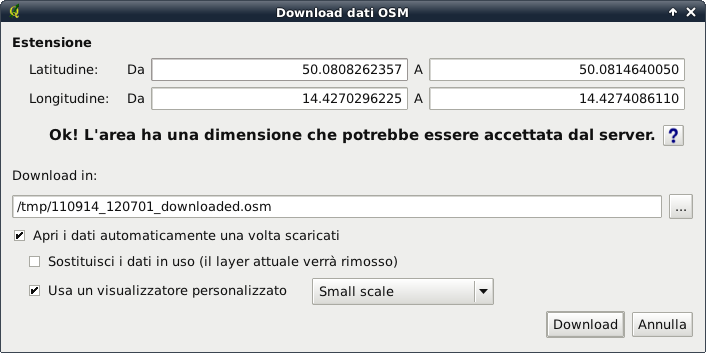
\includegraphics[clip=true, width=8cm]{osm_downloaddialog}
   %\caption{OSM download dialog \nixcaption}\label{fig:osmdownload}
   \caption{Fenêtre de téléchargement de données OSM \nixcaption}\label{fig:osmdownload}
\end{figure}

\begin{description}
%\item[Extent :] Specifies an area to download data from intervals of latitude and longitude degrees. Because there is some restriction of OpenStreetMap server on how much data can be downloaded, the intervals must not be too wide. More detailed info on extent specification can is shown after clicking the \toolbtntwo{osm_questionMark}{help} button on the right.
\item[Emprise :] Spécifie une zone où télécharger les données à partir d'un intervalle de latitude et de longitude en degrés décimaux. Dû aux restrictions sur la quantité de données qui peuvent être téléchargées en une fois depuis le serveur OpenStreetMap, cette zone ne doit pas être trop étendue. Des informations plus détaillées sur cette étendue sont disponibles en cliquant sur le bouton \toolbtntwo{osm_questionMark}{Aide} sur la droite.
%\item[Download to :] Here you are expected to write a path to the file where data will be stored. If you can't remember the structure of your disk, don't panic. The \button{browse} button will help you.
\item[Télécharger vers :] A cet endroit vous devez écrire le chemin vers le fichier où seront stockées les données. Si vous ne vous rappelez pas de la structure de votre disque, ne paniquez pas, le bouton \button{parcourir} est là pour vous aider.
%\item[Open data automatically after download :] Determines, if the download process should be followed by loading the data process or not. If you prefer not to load data now, you can do it later by using the \toolbtntwo{osm_load}{Load OSM from file} button.
\item[Ouvrir les données automatiquement après le téléchargement :] Détermine si le processus de téléchargement doit être suivi de l'affichage des données ou pas. Si vous préférez ne pas afficher les données tout de suite, vous pourrez le faire plus tard en utilisant le bouton \toolbtntwo{osm_load}{Charger OSM depuis un fichier}.
%\item[Replace current data :] This option is active only if \radiobuttonon{Open data automatically after download} is checked. Checking this option means that downloaded data should replace current data we are working with now. Layers of the current data will be removed and new ones will be loaded. When starting QGIS and downloading OSM data for the first time, this option is initially inactive, because there is nothing to replace.
\item[Remplacer les données actuelles :] Cette option est active uniquement si\\ \radiobuttonon{Ouvrir les données automatiquement après le téléchargement} est coché. Cocher l'option signifie que les données téléchargées remplaceront les données courantes. Les couches des données courantes seront retirées et les nouvelles chargées. Au démarrage de QGIS et au premier chargement de données OSM, cette option n'est pas activée, car il n'y a rien à remplacer.
%\item[Use custom renderer :] This option is active only if the \radiobuttonon{Open data automatically after download} checkbox is checked. It determines how many details will be in the map. There are three predefined OSM styles for map displaying. Use \button{Small scale} if you want to view OSM data at low level, to see all details and to edit something. If not you can use \button{Medium scale} or \button{Large scale}. QGIS \CURRENT does not support changing the renderer style dynamically.
\item[Utiliser le moteur de rendu personnalisé :] Cette option est active uniquement si\\ \radiobuttonon{Ouvrir les données automatiquement après le téléchargement} est coché. Elle détermine le niveau de détail de la carte. Il y a trois styles OSM prédéfinis pour l'affichage de la carte. Utilisez \button{Petite échelle} si vous souhaitez visualiser des données à un niveau de zoom très rapproché et pour éditer les données. Sinon, vous pouvez utiliser \button{Échelle intermédiaire} ou \button{Grande échelle}. QGIS \CURRENT ne permet pas de changer de style dynamiquement.
\end{description}

%Click the \button{Download} button to start the download process.
Cliquez sur le bouton \button{Télécharger} pour lancer le processus.

%A progress dialog will continuously inform you about how much of data is already downloaded. When an error occures during the download process, a dialog tells you why. When action finishes succesfully both the progress dialog and download dialog will close themselves.
Une barre de progression vous informera en continu sur la quantité de données déjà téléchargées. Si une erreur se produit pendant le processus de téléchargement, une fenêtre de dialogue vous l'expliquera. Lorsque le téléchargement est terminé, la barre de progression et la fenêtre de téléchargement se fermeront automatiquement.

%\subsection{Uploading OSM data}  
\subsection{Charger des données sur le serveur OSM}  

%Note that the upload is always done on current OSM data. Before opening the OSM Upload dialog, please be sure that you really have the right active layer ~ OSM data.
Notez que le chargement est toujours effectué sur les données OSM courantes. Avant d'ouvrir la fenêtre de dialogue de Chargement OSM, assurez-vous que vous avez la bonne couche OSM active.

%To upload current data to the OSM server click on the \toolbtntwo{osm_upload}{Upload OSM data} button. If there is no such button, OSM toolbar in your QGIS installation is disabled. You can enable it again in \mainmenuopt{Settings} > \mainmenuopt{Toolbars} > \dropmenuopt{OpenStreetMap}. After clicking the \button{upload} button a new dialog will appear.
Pour transférer les données courantes vers le serveur OSM, cliquez sur le bouton \toolbtntwo{osm_upload}{Charger des données OSM}. Si vous ne voyez pas ce bouton, la barre d'outils OSM est peut-être désactivée dans QGIS. Vous pouvez l'activer ou la réactiver dans \mainmenuopt{Vue} > \mainmenuopt{Barres d'outils} > \dropmenuopt{OpenStreetMap}. Après avoir cliqué sur le bouton, une fenêtre de dialogue apparaît.

\begin{figure}[ht]
   \centering
   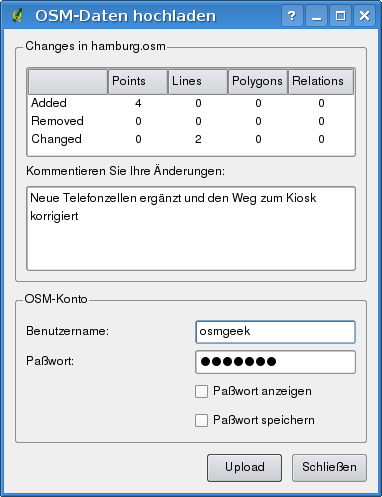
\includegraphics[clip=true, width=8cm]{osm_uploaddialog}
   %\caption{OSM upload dialog \nixcaption}\label{fig:osmupload}
   \caption{Fenêtre de transfert des données vers OSM \nixcaption}\label{fig:osmupload}
\end{figure}

%At the top of the dialog you can check, if you are uploading the correct data. There is a short name of a current database. In the table you find information on how many changes will be uploaded. Statistics are displayed separately for each feature type.
En haut de la fenêtre, vous pouvez vérifier si vous avez sélectionné les bonnes données. Le nom des données courantes est rappelé. Dans le tableau, les informations sur tous les changements à envoyer sont listées. Les statistiques sont disponibles pour chaque type d'entité séparément.

%In the 'Comment on your changes' box you can write brief information on meaning of your upload operation. Just write in brief what data changes you've done or let the box empty.
Dans la zone \og Descriptif de votre changement\fg, vous pouvez décrire brièvement les changements effectués. Décrivez juste brièvement les changements sur les données ou laissez la zone vide.
%Fill 'OSM account' arrays so that the server could authenticate you. If you don't have an account on the OSM server, it's the best time to create one at \url{http://www.openstreetmap.org}. Finally use \button{Upload} to start an upload operation.
Remplissez les informations sur votre \og Compte OSM\fg pour que le serveur puisse vous authentifier. Si vous n'avez pas de compte sur le serveur OSM, c'est le bon moment d'aller en créer un ici : \url{http://www.openstreetmap.org}. Enfin, utilisez le bouton \button{Chargement} pour lancer l'opération.

%\subsection{Saving OSM data}  
\subsection{Sauvegarder des données OSM}  

%To save data from a current map extent to an XML file click on the \toolbtntwo{osm_save}{Save OSM to file} button. If there is no such button, the OSM toolbar in your QuantumGIS installation is probably disabled. You can enable it again in \mainmenuopt{Settings} > \mainmenuopt{Toolbars} > \dropmenuopt{OpenStreetMap}. After clicking on the button a new dialog appears.
Pour sauvegarder les données de la zone de la carte visible vers un fichier XML, cliquez sur le bouton \toolbtntwo{osm_save}{Sauvegarder dans un fichier OSM}. Si vous ne voyez pas ce bouton, la barre d'outils OSM est peut-être désactivée dans QGIS. Vous pouvez l'activer ou la réactiver dans \mainmenuopt{Vue} > \mainmenuopt{Barres d'outils} > \dropmenuopt{OpenStreetMap}. Après avoir cliqué sur le bouton, une fenêtre de dialogue apparaît.

\begin{figure}[ht]
   \centering
   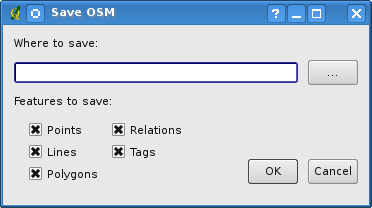
\includegraphics[clip=true, width=8cm]{osm_savedialog}   
   %\caption{OSM saving dialog \nixcaption}\label{fig:osmsave}
   \caption{Fenêtre de sauvegarde de données OSM \nixcaption}\label{fig:osmsave}
\end{figure}

%Select features you want to save into XML file and the file itself. Use the \button{Ok} button to start the operation. The process will create an XML file, in which OSM data from your current map extent are represented. The OSM version of the output file is 0.6. Elements of OSM data (<node>, <way>, <relation>) do not contain information on their changesets and uids. These informations are not compulsory yet, see DTD for OSM XML version 0.6. In the output file OSM elements are not ordered.
Sélectionnez les entités que vous voulez sauvegarder dans un fichier XML ainsi que le fichier lui-même. Utilisez le bouton \button{Ok} pour lancer l'opération. Le processus va créer un fichier XML contenant les données de la zone cartographique courante. La version OSM du fichier de sortie est 0.6. Les éléments des données OSM (<noeud>, <trace>, <relation>) ne contiennent pas les informations sur leur changeset et leur uid. Elles ne sont pas encore obligatoires, voyez le DTD pour la version 0.6 OSM XML. Dans le fichier de sortie, les éléments OSM ne sont pas ordonnés.

%Notice that not only data from the current extent are saved. Into the output file the whole polygons and lines are saved even if only a small part of them is visible in the current extent. For each saved line/polygon all its member nodes are saved too.
Notez que seules les données de la zone géographique courante sont sauvées. Dans le fichier de sortie, même si seule une partie d'un polygone ou d'une ligne sont dans la zone, le polygone ou la ligne dans son entier sont sauvegardés. Pour chaque ligne ou polygone sauvé, tous ses noeuds membres sont également sauvegardés.

%\subsection{Import OSM data}  
\subsection{Importer des données OSM} 

%To import OSM data from an opened non-OSM vector layer follow this instructions: Choose current OSM data by clicking on one of their layers. Click on the \toolbtntwo{osm_import}{Import data from a layer} button. If there is no such button, someone has probably disable the OpenStreetMap toolbar in your QGIS installation. You can enable it again in \mainmenuopt{Settings} > \mainmenuopt{Toolbars} > \dropmenuopt{OpenStreetMap}. 
Pour importer des données OSM depuis une couche vectorielle qui n'est pas au format OSM, suivez ces instructions : choisissez les données OSM courantes en cliquant sur l'une de ses couches. Cliquez sur le bouton \toolbtntwo{osm_import}{Importer des données depuis une couche}. Si vous ne voyez pas ce bouton, la barre d'outils OSM est peut-être désactivée dans QGIS. Vous pouvez l'activer ou la réactiver dans \mainmenuopt{Vue} > \mainmenuopt{Barres d'outils} > \dropmenuopt{OpenStreetMap}.

%After clicking on the button following message may show up:
Après avoir cliqué sur le bouton, le message suivant s'affiche :

\begin{figure}[ht]
   \centering
   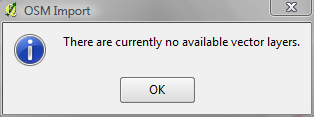
\includegraphics[clip=true, width=8cm]{osm_importdialog}   
   %\caption{OSM import message dialog \nixcaption}\label{fig:osmimportmessage}
   \caption{Fenêtre d'erreur d'importation OSM \nixcaption}\label{fig:osmimportmessage}
\end{figure}

%In such case there is no vector layer currently loaded. The import must be done from a loaded layer - please load a vector layer from which you want to  import data. After a layer is opened, your second try should give you a  better result (don't forget to mark the current OSM layer again):
Dans ce cas, il n'y a pas de couches vectorielles actuellement chargées. L'importation doit se faire depuis une couche vectorielle présente dans QGIS : chargez donc la couche vectorielle dont vous voulez importer les données. Une fois la couche ouverte dans QGIS, réessayez et le résultat devrait être meilleur (n'oubliez pas de sélectionner la couche OSM cible courante) :

\begin{figure}[ht]
   \centering
   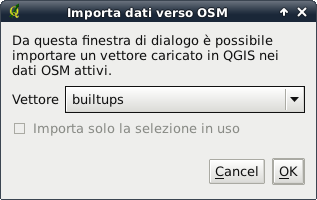
\includegraphics[clip=true, width=8cm]{osm_importtoosmdialog}   
   %\caption{Import data to OSM dialog \nixcaption}\label{fig:osmimporttoosm}
   \caption{Fenêtre d'importation de données vers OSM \nixcaption}\label{fig:osmimporttoosm}
\end{figure}

%Use the submit dialog to start the process of OSM data importing. Reject it if you are not sure you want to import something.
Validez la fenêtre pour lancer le processus d'importation des données vers OSM. Annulez si vous n'êtes pas sûr de vouloir importer des données.

\FloatBarrier
